% !TeX root=../main.tex
\chapter{نتایج}
%\thispagestyle{empty}
\label{chap:results}

\section{مقدمه}

در این فصل، سازوکارهایِ محیط اعتبارسنجی می‌شوند و شکافِ بهینگیِ در دسترسِ سیاست‌هایِ یادگرفته‌شده‌یِ آتی کمّی‌سازی می‌گردد. سه اکتشافیِ حریصانه‌یِ قطعی و یک جوابِ بهینه‌یِ اطلاعاتِ‌کامل که به‌صورتِ دستی محاسبه شده است، در چهار پیکربندیِ محکِ سبدِ پروژه با پیچیدگیِ ساختاریِ فزاینده ارزیابی می‌شوند. این پیکربندی‌ها طوری طراحی شده‌اند که هر یک، یک سازوکارِ مشخص از محیط را مجزا می‌کند — دینامیکِ پیشرفت، زمان‌بندیِ پیش‌پرداخت، ریسکِ فسخ، هماهنگیِ چندپروژه‌ای — که امکانِ انتسابِ دقیقِ حالتِ شکستِ هر اکتشافی را فراهم می‌آورد. تمامیِ قسمت‌ها از طریقِ محیطِ \lr{Gymnasium} توصیف‌شده در بخشِ \ref{sec:problem} اجرا می‌شوند، درحالی‌که دفترِ حسابرسیِ \lr{SQLite} رکوردی کامل از تخصیص‌ها، رویدادهایِ جریانِ نقدی و پرچم‌هایِ نقضِ قانون را به‌ازایِ هر دوره فراهم می‌کند.

\section{محتوا}

% ------------------------------------------------------------
\subsection{پارامترهایِ مشترک}
\label{subsec:shared_params}
% ------------------------------------------------------------

هر چهار پیکربندی، پارامترهایِ قرارداد و محیط را مطابقِ جدولِ \ref{tab:shared_params} به اشتراک می‌گذارند؛ این پارامترها در تمامیِ قسمت‌ها و برایِ تمامیِ حل‌کننده‌ها ثابت نگه داشته شده‌اند تا تفاوت‌هایِ مشاهده‌شده در عملکرد، صرفاً به ساختارِ پیکربندی و سیاستِ حل‌کننده نسبت داده شود.

\begin{table}[H]
  \centering
  % tables/global_params.tex
% tabular only — no table environment, no caption, no label.
% Include in section file as:
%   \input{tables/global_params.tex}
\footnotesize
\renewcommand{\arraystretch}{1.0}
\setlength{\tabcolsep}{3pt}
\rowcolors{2}{RowAlt}{white}
\begin{tabularx}{\textwidth}{llX@{\hspace{6pt}}llX}
  \toprule
  \rowcolor{headbg}
  \multicolumn{1}{c}{\color{headfg}\textbf{Parameter}} &
  \multicolumn{1}{c}{\color{headfg}\textbf{Symbol}} &
  \multicolumn{1}{c}{\color{headfg}\textbf{Value}} &
  \multicolumn{1}{c}{\color{headfg}\textbf{Parameter}} &
  \multicolumn{1}{c}{\color{headfg}\textbf{Symbol}} &
  \multicolumn{1}{c}{\color{headfg}\textbf{Value}} \\
  \midrule
  Retention rate          & $\nu_i$           & 0.05         & Budget tightness        & $\kappa$          & 3.0 \\
  Progress delay cap      & $\delta^{\max}_i$ & 0.15         & Profit margin           & $\pi_i$           & 0.20 \\
  Finish delay cap        & $\Delta^{\max}_i$ & 2 periods    & Discount factor         & $\gamma$          & 0.95 \\
  Termination tolerance   & $\theta_i$        & 2 breach-per.& S-curve shape           & $(a_i,\, b_i)$   & $(1.5,\ 3.0)$ \\
  Annual interest rate    & $r$               & 0.12         & Per-period deficit rate & $r/12$            & 0.01\\
  \bottomrule
\end{tabularx}
  \caption{پارامترهایِ مشترک میانِ تمامیِ پیکربندی‌هایِ محک.
    در هر پرداختِ نقطه‌یِ عطف، بازیافتِ پیش‌پرداخت ابتدا بر رویِ
    پرداختِ ناخالص اعمال می‌شود؛ کسرِ تضمین نیز به‌طورِ مستقل از همان
    پرداختِ ناخالص کسر می‌گردد. تضمینِ انباشته در نقطه‌یِ عطفِ نهایی
    به‌طورِ کامل آزاد می‌شود.}
  \label{tab:shared_params}
\end{table}

\paragraph{قراردادِ مدت.}
پروژه‌ای با مدتِ برنامه‌ریزی‌شده‌یِ $D_i$ در طولِ گام‌هایِ زمانیِ
پروژه، یعنی $\tau_i \in \{0, 1, \ldots, D_i\}$، اجرا می‌شود که
$D_i + 1$ دوره‌یِ فعال را به‌دست می‌دهد. با سقفِ تأخیرِ پایانیِ
$\Delta^{\max}_i = 2$، مهلتِ قطعی در دوره‌یِ $f_i + 2$ از قسمت واقع
می‌شود و هر دنباله‌یِ کارایی دارایِ $D_i + 3$ مدخل است که تمامیِ
دوره‌هایِ فعالِ ممکن را پوشش می‌دهد.

\paragraph{ترتیبِ کسر.}
بازیافتِ پیش‌پرداخت ابتدا بر رویِ پرداختِ ناخالصِ نقطه‌یِ عطف اعمال
می‌شود؛ کسرِ تضمین نیز به‌طورِ مستقل و موازی از همان پرداختِ ناخالص
کسر می‌گردد. در نقطه‌یِ عطفِ نهایی، هرگونه پیش‌پرداختِ بازیافت‌نشده
به‌طورِ کامل تسویه شده و تمامیِ تضمینِ انباشته آزاد می‌شود.

% ------------------------------------------------------------
\subsection{پیکربندی‌هایِ محک}
\label{subsec:configs}
% ------------------------------------------------------------

جدولِ \ref{tab:configs} چهار پیکربندی را خلاصه می‌کند. هر پیکربندی
از یک دنباله‌یِ کاراییِ ترتیبیِ ثابت و سفارشی ($\eta_{i,t}$ که
به‌صورتِ فهرستی قطعی و به‌ازایِ هر پروژه تنظیم شده) تحتِ \lr{seed}
$= 0$ استفاده می‌کند که تکرارپذیریِ دقیق را تضمین می‌نماید.

\begin{table}[H]
  \centering
  % tables/configs.tex
% tabular only — no table environment, no caption, no label.
% Include in section file as:
%   % tables/configs.tex
% tabular only — no table environment, no caption, no label.
% Include in section file as:
%   % tables/configs.tex
% tabular only — no table environment, no caption, no label.
% Include in section file as:
%   \input{tables/configs.tex}
\small
\renewcommand{\arraystretch}{1.3}
\setlength{\tabcolsep}{4pt}
\rowcolors{2}{RowAlt}{white}
\resizebox{\textwidth}{!}{%
\begin{tabular}{lcccccccl}
  \toprule
  \rowcolor{headbg}
  \color{headfg}\textbf{Config} &
  \color{headfg}$N$ &
  \color{headfg}$\mathrm{BAC}_i$ &
  \color{headfg}$D_i$ &
  \color{headfg}$s_i$ &
  \color{headfg}$M_i$ &
  \color{headfg}$\phi_i$ &
  \color{headfg}$\psi^{\mathrm{trig}}_i$ &
  \color{headfg}\textbf{Primary mechanic} \\
  \midrule
  TC-10SF-R
    & 1 & 100         & 0 & 0     & 1 & 0.00 & ---
    & Isolated atom: single action, single milestone \\
  TC-1LMAIF-R
    & 1 & 100         & 3 & 2     & 3 & 0.20 & 0.80
    & Delayed start, progress-triggered advance, high recovery \\
  TC-10MAIF-R
    & 1 & 100         & 3 & 0     & 3 & 0.20 & 0.00
    & Diminishing efficiency, termination risk \\
  TC-3XMAIF-R
    & 3 & 100/200/300 & 3 & 0/6/7 & 3 & 0.20 & 0.00
    & Multi-project, gap then overlap, interacting cash flows \\
  \bottomrule
\end{tabular}%
}
\small
\renewcommand{\arraystretch}{1.3}
\setlength{\tabcolsep}{4pt}
\rowcolors{2}{RowAlt}{white}
\resizebox{\textwidth}{!}{%
\begin{tabular}{lcccccccl}
  \toprule
  \rowcolor{headbg}
  \color{headfg}\textbf{Config} &
  \color{headfg}$N$ &
  \color{headfg}$\mathrm{BAC}_i$ &
  \color{headfg}$D_i$ &
  \color{headfg}$s_i$ &
  \color{headfg}$M_i$ &
  \color{headfg}$\phi_i$ &
  \color{headfg}$\psi^{\mathrm{trig}}_i$ &
  \color{headfg}\textbf{Primary mechanic} \\
  \midrule
  TC-10SF-R
    & 1 & 100         & 0 & 0     & 1 & 0.00 & ---
    & Isolated atom: single action, single milestone \\
  TC-1LMAIF-R
    & 1 & 100         & 3 & 2     & 3 & 0.20 & 0.80
    & Delayed start, progress-triggered advance, high recovery \\
  TC-10MAIF-R
    & 1 & 100         & 3 & 0     & 3 & 0.20 & 0.00
    & Diminishing efficiency, termination risk \\
  TC-3XMAIF-R
    & 3 & 100/200/300 & 3 & 0/6/7 & 3 & 0.20 & 0.00
    & Multi-project, gap then overlap, interacting cash flows \\
  \bottomrule
\end{tabular}%
}
\small
\renewcommand{\arraystretch}{1.3}
\setlength{\tabcolsep}{4pt}
\rowcolors{2}{RowAlt}{white}
\resizebox{\textwidth}{!}{%
\begin{tabular}{lcccccccl}
  \toprule
  \rowcolor{headbg}
  \color{headfg}\textbf{Config} &
  \color{headfg}$N$ &
  \color{headfg}$\mathrm{BAC}_i$ &
  \color{headfg}$D_i$ &
  \color{headfg}$s_i$ &
  \color{headfg}$M_i$ &
  \color{headfg}$\phi_i$ &
  \color{headfg}$\psi^{\mathrm{trig}}_i$ &
  \color{headfg}\textbf{Primary mechanic} \\
  \midrule
  TC-10SF-R
    & 1 & 100         & 0 & 0     & 1 & 0.00 & ---
    & Isolated atom: single action, single milestone \\
  TC-1LMAIF-R
    & 1 & 100         & 3 & 2     & 3 & 0.20 & 0.80
    & Delayed start, progress-triggered advance, high recovery \\
  TC-10MAIF-R
    & 1 & 100         & 3 & 0     & 3 & 0.20 & 0.00
    & Diminishing efficiency, termination risk \\
  TC-3XMAIF-R
    & 3 & 100/200/300 & 3 & 0/6/7 & 3 & 0.20 & 0.00
    & Multi-project, gap then overlap, interacting cash flows \\
  \bottomrule
\end{tabular}%
}
  \caption{خلاصه‌یِ پیکربندی‌هایِ محک. $N$: تعدادِ پروژه‌ها؛
    $D_i$: مدتِ برنامه‌ریزی‌شده؛ $s_i$: شروعِ برنامه‌ریزی‌شده
    (دوره‌یِ قسمت)؛ $M_i$: نقاطِ عطفِ غیرِپیش‌پرداخت؛ $\phi_i$: نرخِ
    پیش‌پرداخت؛ $\psi^{\mathrm{trig}}_i$: سطحِ پیشرفتی که در آن
    پیش‌پرداخت پرداخت می‌شود (۰٫۰۰ به‌معنایِ شروعِ پروژه است).}
  \label{tab:configs}
\end{table}

\paragraph{\lr{TC-10SF-R} --- اتمِ مجزا.}
یک پروژه، یک نقطه‌یِ عطفِ غیرِپیش‌پرداخت، بدونِ پیش‌پرداخت، با
مدتِ برنامه‌ریزی‌شده‌یِ $D_i = 0$. این پروژه تنها یک اقدامِ
برنامه‌ریزی‌شده در $\tau_i = 0$ دارد و مهلتِ قطعیِ آن در دوره‌یِ ۲
از قسمت واقع می‌شود. قیمتِ قرارداد $P_i = 120$ است و تنها نقطه‌یِ
عطف وزنِ $w = 1.0$ را دارد. جدولِ \ref{tab:tc10sf} ردِ پرداختِ
نقطه‌یِ عطف را برایِ این پیکربندی تشریح می‌کند.

\begin{table}[H]
  \centering
  % tables/tc_10sf_r.tex
% tabular only — no table environment, no caption, no label.
\footnotesize
\renewcommand{\arraystretch}{1.3}
\setlength{\tabcolsep}{7pt}
\rowcolors{2}{RowAlt}{white}
\begin{tabularx}{\textwidth}{cXrrrrr}
  \toprule
  \rowcolor{headbg}
  \multicolumn{1}{c}{\color{headfg}\textbf{Milestone}} &
  \multicolumn{1}{c}{\color{headfg}\textbf{Weight}} &
  \multicolumn{1}{c}{\color{headfg}\textbf{Gross}} &
  \multicolumn{1}{c}{\color{headfg}\textbf{Adv.\ Recov.}} &
  \multicolumn{1}{c}{\color{headfg}\textbf{Adv.\ Remaining}} &
  \multicolumn{1}{c}{\color{headfg}\textbf{Retention}} &
  \multicolumn{1}{c}{\color{headfg}\textbf{Net}} \\
  \midrule
  $j=1$ & $1.00$ & $120$ & $0.0$ & $0.0$ & $-6.0$ $(\to +6.0)$ & $120.0$ \\
  \midrule
  \rowcolor{white}
  \multicolumn{2}{l}{\textbf{Total}} & $\mathbf{120}$ & $\mathbf{0.0}$ & --- & $\mathbf{0.0}$ & $\mathbf{120.0}$ \\
  \bottomrule
\end{tabularx}
  \caption{\lr{TC-10SF-R}: ردِ پرداختِ نقطه‌یِ عطف. تضمین کسر شده
    و بلافاصله در نقطه‌یِ عطفِ نهایی آزاد می‌شود که پرداختِ خالصِ
    $= 120$ را بدونِ هیچ کسرِ پیش‌پرداختی به‌دست می‌دهد.}
  \label{tab:tc10sf}
\end{table}

\paragraph{\lr{TC-1LMAIF-R} --- شروعِ تأخیری و پیش‌پرداختِ محرک‌شونده با پیشرفت.}
یک پروژه با شروعِ برنامه‌ریزی‌شده‌یِ $s_i = 2$، مدتِ
برنامه‌ریزی‌شده‌یِ $D_i = 3$ (چهار دوره‌یِ فعال: $\tau_i \in
\{0,1,2,3\}$)، سه نقطه‌یِ عطفِ غیرِپیش‌پرداخت، و نرخِ پیش‌پرداختِ
$\phi_i = 0.20$ با محرکِ $\psi^{\mathrm{trig}}_i = 0.80$. پیش‌پرداختِ
$\phi_i \times P_i = 24$ تنها زمانی پرداخت می‌شود که پیشرفتِ تجمعیِ
$EV_{i,t} \geq 0.80$ محقق شود. نرخِ بازیافتِ پیش‌پرداختِ $\rho_i =
0.50$ بالاترین مقدار در مجموعه‌یِ محک است. دنباله‌یِ کارایی:
$[0.91,\, 1.17,\, 0.83,\, 0.91,\, 1.17,\, 0.83]$. جدولِ
\ref{tab:tc1lmaif} ردِ کاملِ پرداخت را نشان می‌دهد.

\begin{table}[H]
  \centering
  % tables/tc_1lmaif_r.tex
% tabular only — no table environment, no caption, no label.
\footnotesize
\renewcommand{\arraystretch}{1.3}
\setlength{\tabcolsep}{7pt}
\rowcolors{2}{RowAlt}{white}
\begin{tabularx}{\textwidth}{cXrrrrr}
  \toprule
  \rowcolor{headbg}
  \multicolumn{1}{c}{\color{headfg}\textbf{Milestone}} &
  \multicolumn{1}{c}{\color{headfg}\textbf{Gross}} &
  \multicolumn{1}{c}{\color{headfg}\textbf{Adv.\ Recov.}} &
  \multicolumn{1}{c}{\color{headfg}\textbf{Adv.\ Remaining}} &
  \multicolumn{1}{c}{\color{headfg}\textbf{Retention}} &
  \multicolumn{1}{c}{\color{headfg}\textbf{Ret.\ Release}} &
  \multicolumn{1}{c}{\color{headfg}\textbf{Net}} \\
  \midrule
  $j=1$ & $18.0$ & $9.0$  & $15.0$ & $-0.9$ & $0.0$  & $8.1$  \\
  $j=2$ & $42.0$ & $15.0$ & $0.0$  & $-2.1$ & $0.0$  & $24.9$ \\
  $j=3$ & $60.0$ & $0.0$  & $0.0$  & $-3.0$ & $+6.0$ & $63.0$ \\
  \midrule
  \rowcolor{white}
  \multicolumn{1}{l}{\textbf{Total}} & $\mathbf{120}$ & $\mathbf{24.0}$ & --- & $\mathbf{-6.0}$ & $\mathbf{+6.0}$ & $\mathbf{96.0}$ \\
  \bottomrule
\end{tabularx}
  \caption{\lr{TC-1LMAIF-R}: ردِ پرداختِ نقطه‌یِ عطف شاملِ بازیافتِ
    پیش‌پرداخت و کسرِ تضمین. تضمین به‌طورِ کامل ($6.0$) در نقطه‌یِ
    عطفِ $j=3$ آزاد می‌شود.}
  \label{tab:tc1lmaif}
\end{table}

\paragraph{\lr{TC-10MAIF-R} --- کاهشِ کارایی و ریسکِ فسخ.}
یک پروژه با شروعِ برنامه‌ریزی‌شده‌یِ $s_i = 0$، مدتِ
برنامه‌ریزی‌شده‌یِ $D_i = 3$، سه نقطه‌یِ عطف، نرخِ پیش‌پرداختِ
$\phi_i = 0.20$ که در شروعِ پروژه پرداخت می‌شود
($\psi^{\mathrm{trig}}_i = 0.00$)، و نرخِ بازیافتِ $\rho_i = 0.20$.
دنباله‌یِ کارایی به‌طورِ یکنواخت کاهشی است:
$[0.95,\, 0.91,\, 0.55,\, 0.40,\, 0.30,\, 0.20]$. پیش‌پرداختِ $24$
در $t = 0$ پرداخت می‌شود. جدولِ \ref{tab:tc10maif} ردِ پرداختِ
نقطه‌یِ عطف را تشریح می‌کند؛ این پیکربندی سازوکارِ فسخ را تحتِ فشار
قرار می‌دهد، چرا که افتِ شدیدِ کارایی، حفظِ $\delta_{i,t} \leq
\delta^{\max}_i = 0.15$ را به‌تدریج پرهزینه‌تر می‌کند.

\begin{table}[H]
  \centering
  % tables/tc_10maif_r.tex
% tabular only — no table environment, no caption, no label.
\footnotesize
\renewcommand{\arraystretch}{1.3}
\setlength{\tabcolsep}{7pt}
\rowcolors{2}{RowAlt}{white}
\begin{tabularx}{\textwidth}{cXrrrrr}
  \toprule
  \rowcolor{headbg}
  \multicolumn{1}{c}{\color{headfg}\textbf{Milestone}} &
  \multicolumn{1}{c}{\color{headfg}\textbf{Gross}} &
  \multicolumn{1}{c}{\color{headfg}\textbf{Adv.\ Recov.}} &
  \multicolumn{1}{c}{\color{headfg}\textbf{Adv.\ Remaining}} &
  \multicolumn{1}{c}{\color{headfg}\textbf{Retention}} &
  \multicolumn{1}{c}{\color{headfg}\textbf{Ret.\ Release}} &
  \multicolumn{1}{c}{\color{headfg}\textbf{Net}} \\
  \midrule
  $j=1$ & $18.0$ & $3.6$  & $20.4$ & $-0.9$ & $0.0$  & $13.5$ \\
  $j=2$ & $42.0$ & $8.4$  & $12.0$ & $-2.1$ & $0.0$  & $31.5$ \\
  $j=3$ & $60.0$ & $12.0$ & $0.0$  & $-3.0$ & $+6.0$ & $51.0$ \\
  \midrule
  \rowcolor{white}
  \multicolumn{1}{l}{\textbf{Total}} & $\mathbf{120}$ & $\mathbf{24.0}$ & --- & $\mathbf{-6.0}$ & $\mathbf{+6.0}$ & $\mathbf{96.0}$ \\
  \bottomrule
\end{tabularx}
  \caption{\lr{TC-10MAIF-R}: ردِ پرداختِ نقطه‌یِ عطف. پیش‌پرداختِ
    $24$ در $t=0$ پرداخت می‌شود؛ نرخِ بازیافتِ $\rho_i = 0.20$.}
  \label{tab:tc10maif}
\end{table}

\paragraph{\lr{TC-3XMAIF-R} --- چندپروژه‌ای با شکاف و هم‌پوشانی.}
سه پروژه با مقیاسِ ناهمگن ($\mathrm{BAC}_i = [100,\, 200,\, 300]$،
قیمت‌هایِ $[120,\, 240,\, 360]$) و شروع‌هایِ پلکانی ($s_i = [0,\,
6,\, 7]$). هر پروژه مدتِ برنامه‌ریزی‌شده‌یِ $D_i = 3$، سه نقطه‌یِ
عطف، و نرخِ پیش‌پرداختِ $\phi_i = 0.20$ را دارد که در شروعِ پروژه
پرداخت می‌شود. این قسمت دارایِ دو فازِ متمایز از نظرِ ساختاری است:
یک \emph{فازِ شکاف} ($t = 4,\,5$) که در آن هیچ تخصیصی لازم نیست و
بودجه انباشته می‌شود، و یک \emph{فازِ هم‌پوشانی} ($t = 7,\,8,\,9$)
که در آن پروژه‌هایِ ۱ و ۲ به‌طورِ هم‌زمان برایِ ذخیره‌یِ مشترکِ $B_t$
رقابت می‌کنند. جدولِ \ref{tab:tc3xmaif_projects} پارامترهایِ هر
پروژه و دنباله‌هایِ کارایی را خلاصه می‌کند و جدولِ
\ref{tab:tc3xmaif_advances} برنامه‌یِ خروجیِ پیش‌پرداخت را تشریح
می‌کند.

\begin{table}[H]
  \centering
  % tables/tc_3xmaif_r_projects.tex
% tabular only — no table environment, no caption, no label.
\footnotesize
\renewcommand{\arraystretch}{1.3}
\setlength{\tabcolsep}{7pt}
\rowcolors{2}{RowAlt}{white}
\begin{tabularx}{\textwidth}{crrrrrrX}
  \toprule
  \rowcolor{headbg}
  \multicolumn{1}{c}{\color{headfg}\textbf{Project}} &
  \multicolumn{1}{c}{\color{headfg}$\mathrm{BAC}_i$} &
  \multicolumn{1}{c}{\color{headfg}$P_i$} &
  \multicolumn{1}{c}{\color{headfg}$s_i$} &
  \multicolumn{1}{c}{\color{headfg}$D_i$} &
  \multicolumn{1}{c}{\color{headfg}$M_i$} &
  \multicolumn{1}{c}{\color{headfg}$\phi_i$} &
  \multicolumn{1}{c}{\color{headfg}\textbf{Efficiency sequence $\eta_{i,t}$}} \\
  \midrule
  0 & $100$ & $120$ & $0$ & $3$ & $3$ & $0.20$ & $[0.91,\ 1.17,\ 0.83,\ 0.91,\ 1.17,\ 0.83]$ \\
  1 & $200$ & $240$ & $6$ & $3$ & $3$ & $0.20$ & $[1.09,\ 0.84,\ 1.18,\ 1.09,\ 0.84,\ 1.18]$ \\
  2 & $300$ & $360$ & $7$ & $3$ & $3$ & $0.20$ & $[0.97,\ 1.13,\ 0.86,\ 0.97,\ 1.13,\ 0.86]$ \\
  \bottomrule
\end{tabularx}
  \caption{\lr{TC-3XMAIF-R}: پارامترهایِ هر پروژه و دنباله‌هایِ
    کارایی. هیچ‌یک از دنباله‌ها به‌طورِ یکنواخت کاهشی نیست؛ چالش،
    صرفاً هماهنگی و زمان‌بندیِ جریانِ نقدی است.}
  \label{tab:tc3xmaif_projects}
\end{table}

\begin{table}[H]
  \centering
  % tables/tc_3xmaif_r_advances.tex
% tabular only — no table environment, no caption, no label.
\footnotesize
\renewcommand{\arraystretch}{1.3}
\setlength{\tabcolsep}{7pt}
\rowcolors{2}{RowAlt}{white}
\begin{tabularx}{\textwidth}{cXrrr}
  \toprule
  \rowcolor{headbg}
  \multicolumn{1}{c}{\color{headfg}\textbf{Episode period $t$}} &
  \multicolumn{1}{c}{\color{headfg}\textbf{Event}} &
  \multicolumn{1}{c}{\color{headfg}\textbf{Project}} &
  \multicolumn{1}{c}{\color{headfg}\textbf{Advance outflow}} &
  \multicolumn{1}{c}{\color{headfg}\textbf{Cumulative outflow}} \\
  \midrule
  $t = 0$ & Project 0 start  & 0 & $-24$ & $-24$  \\
  $t = 3$ & Project 0 finish & 0 & ---   & $-24$  \\
  $t = 4$ & Gap phase begins & --- & ---  & $-24$  \\
  $t = 5$ & Gap phase ends   & --- & ---  & $-24$  \\
  $t = 6$ & Project 1 start  & 1 & $-48$ & $-72$  \\
  $t = 7$ & Project 2 start  & 2 & $-72$ & $-144$ \\
  \bottomrule
\end{tabularx}
  \caption{\lr{TC-3XMAIF-R}: برنامه‌یِ خروجیِ پیش‌پرداخت. خروجی‌هایِ
    هم‌زمان در $t=6$ و $t=7$ بزرگ‌ترین کسریِ تک‌دوره‌ای را در
    مجموعه‌یِ محک تولید می‌کنند.}
  \label{tab:tc3xmaif_advances}
\end{table}

% ------------------------------------------------------------
\subsection{حل‌کننده‌ها}
\label{subsec:solvers}
% ------------------------------------------------------------

چهار روش ارزیابی می‌شوند که تعریفِ رسمیِ آن‌ها در بخشِ
\ref{subsubsec:baselines} آمده است.

\textbf{\lr{Reach-Plan}} ($\pi^{\mathrm{rp}}$) مقدارِ
$x^{\mathrm{rp}}_{i,t}$ را تخصیص می‌دهد تا هر پروژه‌یِ فعال را در هر
دوره دقیقاً به پیشرفتِ برنامه‌ریزی‌شده‌یِ منحنیِ \lr{S} برساند،
صرف‌نظر از کمیابیِ بودجه یا نزدیکیِ نقطه‌یِ عطف.

\textbf{\lr{Catchup-T}} ($\pi^{\mathrm{cu}}$) کمینه‌یِ مخارجِ
$x^{\mathrm{cu}}_{i,t}$ لازم برایِ نگه‌داشتنِ تأخیرِ پیشرفت در
محدوده‌یِ $\delta^{\max}_i$ در همین دوره را تخصیص می‌دهد و
بدین‌ترتیب بودجه را برایِ دوره‌هایِ بعدی و سایرِ پروژه‌ها حفظ
می‌کند.

\textbf{\lr{Catchup-Next-T}} ($\pi^{\mathrm{cu}+1}$) به‌صورتِ
پیش‌دستانه مقدارِ $x^{\mathrm{cu}+1}_{i,t}$ را تخصیص می‌دهد تا
تأخیرِ پیش‌بینی‌شده در دوره‌یِ بعد نیز در محدوده‌یِ
$\delta^{\max}_i$ باقی بماند، به بهایِ مخارجِ اولیه‌یِ بالاتر.

\textbf{بهینه‌یِ اطلاعاتِ‌کامل} ($\pi^*$) با دانشِ پیشینِ کاملِ
تمامیِ تحقق‌هایِ کاراییِ $(\eta_{i,t})$ و از طریقِ واسطِ تعاملیِ
\code{play.py} با دنباله‌هایِ کاراییِ از پیش ثابت‌شده، به‌صورتِ
دستی محاسبه می‌شود. این مقدار نقشِ مرجعِ کرانِ بالاییِ $Z^*$ را از
گزاره‌یِ \ref{prop:upper_bound} ایفا می‌کند. پیاده‌سازیِ یک
حل‌کننده‌یِ الگوریتمیِ قابل‌حل (برنامه‌ریزیِ خطی یا برنامه‌ریزیِ
پویا) به‌عنوانِ کارِ آینده باقی گذاشته شده است؛ محاسبه‌یِ دستی
برایِ تعیینِ سقفِ عملکرد در چهار پیکربندیِ موردِمطالعه در این‌جا
کافی است.

هر چهار روش تحتِ \lr{seed} $= 0$ و با دنباله‌هایِ کاراییِ ترتیبیِ
ثابت و سفارشیِ مشخص‌شده در بالا ارزیابی می‌شوند که تکرارپذیریِ دقیق
را در تمامیِ اجراها و حل‌کننده‌ها تضمین می‌کند.

\begin{figure}[H]
  \centering
  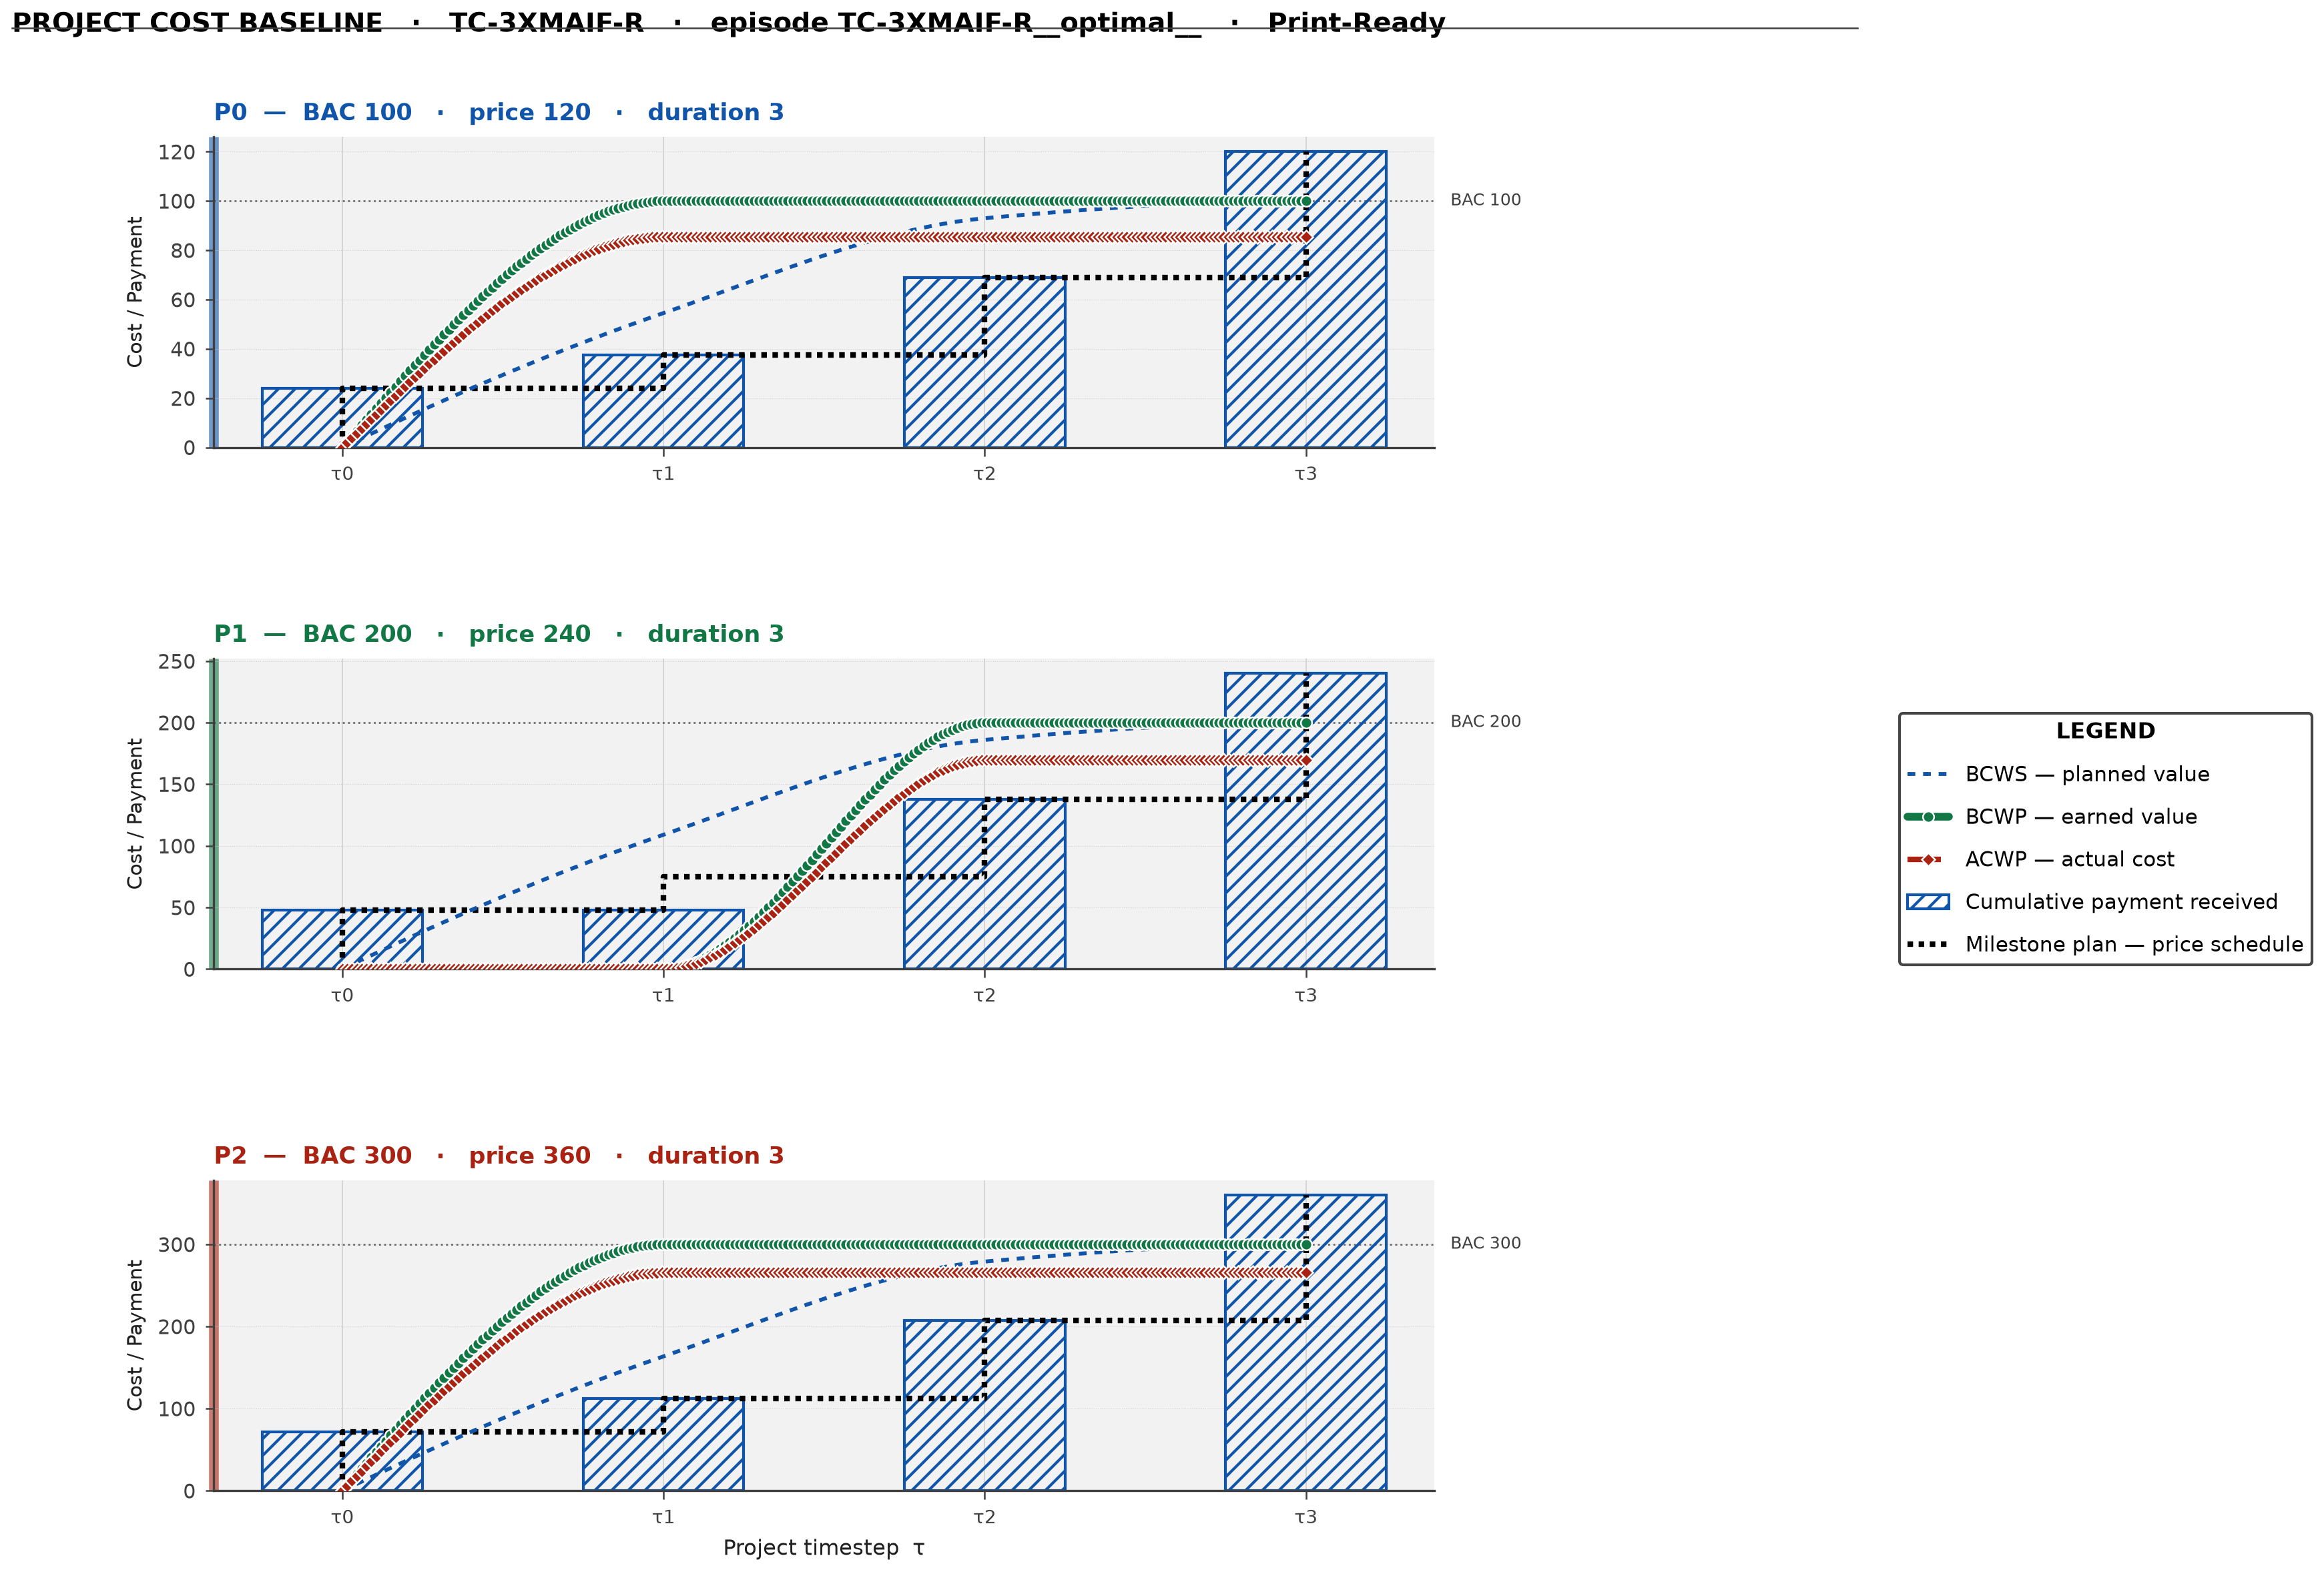
\includegraphics[width=\textwidth]{figures/01c_cost_baseline_E.png}
  \caption{خطِ پایه‌یِ هزینه برایِ پیکربندیِ \lr{TC-3XMAIF-R} تحتِ
    جوابِ بهینه.}
  \label{fig:cost_baseline_three}
\end{figure}

% ------------------------------------------------------------
\subsection{نتایج}
\label{subsec:results}
% ------------------------------------------------------------

شکلِ \ref{fig:gap_plot} ارزشِ خالصِ فعلیِ تجمعیِ قسمت $G =
\sum_{t=0}^{T} \gamma^t \Delta B_t$ را برایِ هر روش در چهار
پیکربندی، به‌ترتیبِ پیچیدگیِ ساختاریِ فزاینده، گزارش می‌کند.

\begin{figure}[H]
  \centering
  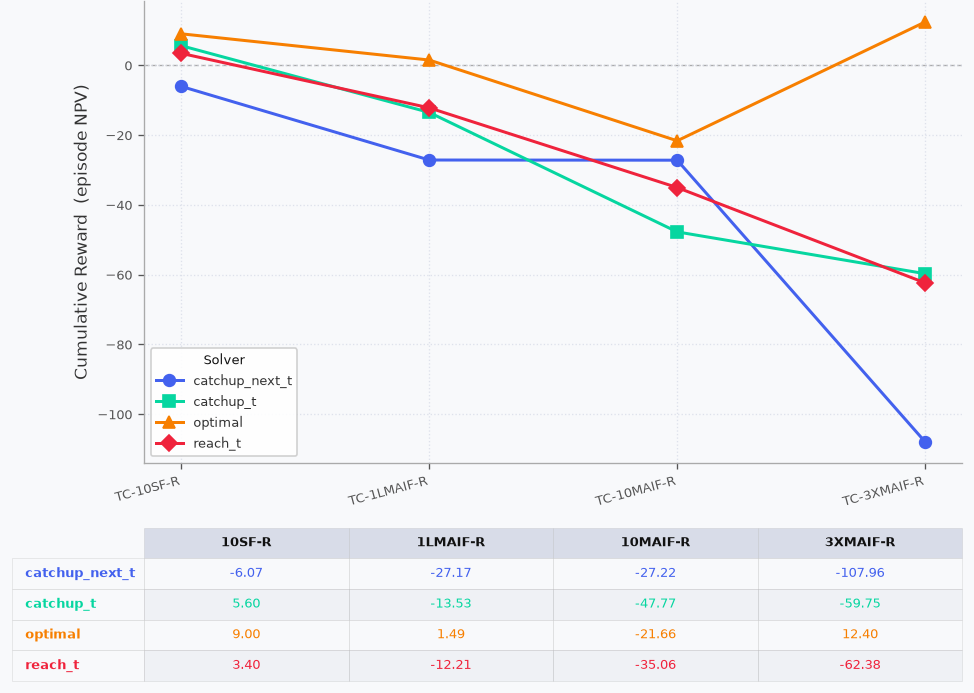
\includegraphics[width=\textwidth]{figures/gap_plot.png}
  \caption{ارزشِ خالصِ فعلیِ تجمعیِ قسمتِ $G$ برایِ سه اکتشافیِ
    حریصانه‌یِ قطعی و بهینه‌یِ اطلاعاتِ‌کامل، در چهار پیکربندیِ
    محک به‌ترتیبِ پیچیدگیِ فزاینده‌یِ سبدِ پروژه. گستردگیِ فزاینده‌یِ
    شکاف تأیید می‌کند که تخصیصِ مبتنی‌بر قاعده، به‌طورِ سیستماتیک با
    افزایشِ پیچیدگیِ ساختاری تضعیف می‌شود.}
  \label{fig:gap_plot}
\end{figure}

\paragraph{\lr{TC-10SF-R}.}
در پیکربندیِ تک‌دوره‌ایِ مجزا، هر سه اکتشافی ارزشِ خالصِ فعلیِ مثبت
تولید می‌کنند و شکاف ناچیز است. \lr{Reach-Plan} به مقدارِ $5.60$ در
برابرِ بهینه‌یِ $9.00$ می‌رسد (شکافِ $3.40$)؛ \lr{Catchup-T} با
$3.40$ در پیِ آن است. \lr{Catchup-Next-T} با $-6.07$ به پایان
می‌رسد: با تنها یک دوره‌یِ فعال و یک نقطه‌یِ عطف، پیش‌بینیِ
یک‌دوره‌ایِ آن بیش از آنچه نقطه‌یِ عطف نیاز دارد مخارج می‌کند و
بدونِ بازگشتِ جبران‌کننده، هزینه‌یِ بهره را متحمل می‌شود. این نتیجه
تأیید می‌کند که محیط، تخصیصِ محافظه‌کارانه‌یِ مازاد را به‌درستی
به‌عنوانِ زیانِ خالص قیمت‌گذاری می‌کند.

\paragraph{\lr{TC-1LMAIF-R}.}
پیش‌پرداختِ محرک‌شونده با پیشرفت و نرخِ بازیافتِ بالا ($\rho_i =
0.50$) بلافاصله پس از فعال‌شدنِ پیش‌پرداخت، یک فرورفتگیِ نقدینگی
ایجاد می‌کند. هر سه اکتشافی ارزشِ خالصِ فعلیِ منفی تولید می‌کنند،
درحالی‌که بهینه با $1.49$ به‌صورتِ جزئی مثبت باقی می‌ماند؛ شکافِ
بهترین‌اکتشافی $14.70$ است. بهینه‌یِ اطلاعاتِ‌کامل با بهره‌گیری از
دنباله‌یِ کاراییِ شناخته‌شده، زمان‌بندیِ تأییدِ نقاطِ عطف را طوری
تنظیم می‌کند که محرکِ پیش‌پرداخت در مناسب‌ترین لحظه فعال شود و
کسرهایِ بزرگِ بازیافت در $j = 1$ ($-9.0$) و $j = 2$ ($-15.0$) با
ورودی‌هایِ نقدیِ بعدی جبران شوند. سیاست‌هایِ حریصانه که تنها بر
اساسِ سیگنال‌هایِ دوره‌یِ جاری تخصیص می‌دهند، نمی‌توانند زمان‌بندیِ
محرک را پیش‌بینی کنند و در دوره‌یِ کم‌بازده پیش از فعال‌شدنِ
پیش‌پرداخت، بیش از حد تخصیص می‌دهند. هر دویِ $\pi^{\mathrm{rp}}$ و
$\pi^{\mathrm{cu}}$ به ارزشِ خالصِ فعلیِ یکسانی ($-13.21$) می‌رسند
که نشان می‌دهد قیدِ الزام‌آور، سقفِ تأخیر نیست بلکه زمان‌بندیِ
پرداخت است: هر دو قاعده، تلورانس را در دوره‌هایِ یکسان برآورده
می‌کنند، اما هیچ‌یک تخصیص را به‌درستی زمان‌بندی نمی‌کند تا ورودیِ
پیش‌پرداخت را زودتر دریافت کند.

\paragraph{\lr{TC-10MAIF-R}.}
دنباله‌یِ کاراییِ یکنواخت‌کاهشی، مسئله‌یِ زمان‌بندیِ تخصیص را حاد
می‌کند. حتی بهینه‌یِ اطلاعاتِ‌کامل نیز تنها به $-21.66$ می‌رسد:
فروپاشیِ کاراییِ مراحلِ پایانی ($\eta_{i,t} = 0.30,\, 0.20$)
بازیابیِ کاملِ پروژه را غیرِاقتصادی می‌کند. \lr{Catchup-Next-T}
($-27.22$) از هر دویِ \lr{Reach-Plan} ($-35.06$) و \lr{Catchup-T}
($-47.77$) بهتر عمل می‌کند: پیش‌بینیِ ریسک‌گریزِ آن، کار را به
دوره‌هایِ اولیه‌یِ پرکارایی منتقل می‌کند و مخارج را در دوره‌هایِ
پایانیِ تقریباً غیرِمؤثر، که در آن‌ها هر واحد تخصیص پیشرفتِ ناچیزی
به‌همراه دارد، کاهش می‌دهد. \lr{Catchup-T} بدترین عملکرد را دارد
زیرا قاعده‌یِ حداقلِ‌مخارجِ آن، تخصیص را در دوره‌هایِ کم‌کارایی
برایِ حفظِ کفِ تلورانس ادامه می‌دهد و هزینه را بدونِ پیشرفتِ
معناداری انباشته می‌کند. شکافِ بهترین‌اکتشافیِ $5.56$، کوچک‌ترین
مقدار در مجموعه است، زیرا چالشِ این‌جا زمان‌بندیِ کاراییِ سطحِ
پروژه است و نه هماهنگیِ چندپروژه‌ای.

\paragraph{\lr{TC-3XMAIF-R}.}
پیکربندیِ چندپروژه‌ای، بارزترین نتیجه را تولید می‌کند. بهینه‌یِ
اطلاعاتِ‌کامل به $+12.40$ می‌رسد: با دنباله‌هایِ کاراییِ
شناخته‌شده، عرّاف زمان‌بندیِ پرداختِ پیش‌پرداخت‌ها، تأییدِ نقاطِ
عطف، و انباشتِ بودجه در فازِ شکاف را طوری تنظیم می‌کند که سبدِ
پیچیده را به یک قسمتِ سودآور تبدیل کند. هر اکتشافیِ حریصانه زیان
تولید می‌کند — \lr{Reach-Plan} با $-59.75$، \lr{Catchup-T} با
$-62.38$، \lr{Catchup-Next-T} با $-107.96$ — و شکافِ
بهترین‌اکتشافی به $72.15$ می‌رسد که افزایشی $21$ برابری نسبت به
\lr{TC-10SF-R} است. معکوس‌شدنِ علامت (بهینه‌یِ سودآور،
اکتشافی‌هایِ زیان‌ده) مشاهده‌یِ محوری است. خروجی‌هایِ هم‌زمانِ
پیش‌پرداخت در $t = 6$ ($-48$) و $t = 7$ ($-72$) کسریِ مشترکِ بزرگی
ایجاد می‌کنند که هر قاعده‌یِ حریصانه‌یِ تک‌پروژه‌ای آن را به‌طورِ
مستقل مدیریت می‌کند، بدونِ در‌نظرگرفتنِ این‌که تخصیصِ خودش چگونه
ذخیره‌یِ در‌دسترسِ پروژه‌یِ هم‌زمان را تحلیل می‌برد.
\lr{Catchup-Next-T} به $-107.96$ سقوط می‌کند زیرا مخارجِ
پیش‌دستانه‌یِ تهاجمیِ آن در هر سه پروژه‌یِ هم‌زمان‌فعال، بودجه را
در طولِ فازِ هم‌پوشانی تمام می‌کند و ذخیره‌یِ کافی برایِ تأییدِ
نقاطِ عطفِ پایانیِ پرارزشِ پروژه‌هایِ ۱ و ۲ باقی نمی‌گذارد.

\section{اعتبارسنجی}

سازوکارهایِ محیط از طریقِ مقایسه‌یِ عملکردِ سه اکتشافیِ قطعی با
کرانِ بالایِ نظریِ اطلاعاتِ‌کامل (گزاره‌یِ \ref{prop:upper_bound})
اعتبارسنجی می‌شوند؛ این مقایسه، نوعی سه‌سویه‌سازی
\lr{(triangulation)} میانِ جوابِ تحلیلیِ بالادست، سیاست‌هایِ
قاعده‌محورِ ساده، و رکوردِ کاملِ دفترِ حسابرسیِ \lr{SQLite} فراهم
می‌کند. تکرارپذیریِ دقیق (ثابت‌بودنِ \lr{seed} و دنباله‌هایِ کارایی
در تمامیِ اجراها) پایاییِ \lr{(reliability)} نتایج را تضمین
می‌کند، درحالی‌که تطابقِ رفتارِ هر پیکربندی با سازوکارِ
موردِانتظارش (پیشرفت، زمان‌بندیِ پیش‌پرداخت، فسخ، هماهنگیِ
چندپروژه‌ای) اعتبارِ \lr{(validity)} مدل‌سازی را نشان می‌دهد. سه
یافته‌یِ کلیدی از این مطالعه به‌دست می‌آید.

\paragraph{شکاف به‌طورِ یکنواخت با پیچیدگیِ ساختاری افزایش می‌یابد.}
شکافِ بهترین‌اکتشافی از $3.40$ (\lr{TC-10SF-R}) به $14.70$
(\lr{TC-1LMAIF-R}) و سپس به $72.15$ (\lr{TC-3XMAIF-R}) افزایش
می‌یابد؛ افزایشی $21$ برابری از ساده‌ترین تا پیچیده‌ترین
پیکربندی. \lr{TC-10MAIF-R} ($5.56$) تنها استثنا نسبت به
یکنواختیِ کامل است: چالشِ آن زمان‌بندیِ کاراییِ سطحِ پروژه است،
نه هماهنگیِ چندپروژه‌ای، از همین رو شکافِ آن با وجودِ دشواریِ
بالاترِ درون‌پروژه‌ای، کوچک‌تر از \lr{TC-1LMAIF-R} است. شکاف در
\lr{TC-3XMAIF-R} تنزلِ جزئی نیست؛ بلکه بازتابِ یک شکستِ ساختاری در
تخصیصِ حریصانه تحتِ الزاماتِ هماهنگیِ بودجه‌یِ مشترک است که هیچ
قاعده‌یِ تک‌پروژه‌ای قادر به حلِ آن نیست.

\paragraph{هیچ اکتشافیِ واحدی چیره نیست.}
هر اکتشافی دستِ‌کم در یک پیکربندی بهترین عملکرد را دارد:
\lr{Reach-Plan} در \lr{TC-10SF-R}، \lr{Catchup-Next-T} در
\lr{TC-10MAIF-R}، \lr{Catchup-T} در \lr{TC-3XMAIF-R}. این امر
تأیید می‌کند که سیاستِ بهینه انطباقی است: تخصیصِ درست به‌طورِ
هم‌زمان به مسیرِ کارایی، ساختارِ پرداختِ نقطه‌یِ عطف، زمان‌بندیِ
محرکِ پیش‌پرداخت، و فازبندیِ پروژه‌هایِ هم‌زمان بستگی دارد —
ترکیبی که هیچ قاعده‌یِ ثابتی قادر به دربرگرفتنِ آن نیست. حالتِ
شکستِ هر اکتشافی به یک ویژگیِ ساختاریِ مشخص قابلِ انتساب است:
\lr{Reach-Plan} در مجموع بیش از حد مخارج می‌کند؛ \lr{Catchup-T}
پیش‌بینیِ ناکافی دارد؛ \lr{Catchup-Next-T} در فازِ هم‌پوشانیِ
چندپروژه‌ای بیش از حد متعهد می‌شود.

\paragraph{هدفِ بهبودِ به‌خوبی‌تعریف‌شده‌ای برایِ عامل‌هایِ یادگرفته‌شده وجود دارد.}
بهینه‌یِ اطلاعاتِ‌کامل $G(\pi^*)$ یک کرانِ بالاییِ مشخص (گزاره‌یِ
\ref{prop:upper_bound}) را برایِ هر پیکربندی فراهم می‌کند. در
\lr{TC-3XMAIF-R}، نوسان میانِ بهترینِ دست‌یافتنی ($+12.40$) و
بهترینِ حریصانه ($-59.75$) برابرِ $72.15$ واحدِ ارزشِ خالصِ فعلی
است — تفاوتِ میانِ یک نتیجه‌یِ سودآور و یک نتیجه‌یِ عمیقاً زیان‌ده
برایِ سبد. بدین‌ترتیب سازوکارهایِ محیط به‌طورِ تجربی اعتبارسنجی
می‌شوند: هر پیکربندی الگویِ موردِانتظارِ رویدادهایِ جریانِ نقدی
(پرداختِ پیش‌پرداخت، تأییدِ نقاطِ عطف، کسرِ بازیافت، آزادسازیِ
تضمین، تعلقِ بهره) را به‌درستی و با توالیِ صحیح و سازگاریِ مالی
تولید می‌کند، و بهینه‌یِ اطلاعاتِ‌کامل از ویژگی‌هایِ ساختاری‌ای
بهره می‌گیرد که قواعدِ حریصانه از نظرِ معماری قادر به دسترسی به
آن‌ها نیستند. این شکاف، ارزشِ تخصیصِ هوشمندِ ترتیبی است و هدفِ
عملکردی برایِ عامل‌هایِ یادگیریِ تقویتیِ آتی است که بر رویِ
محیطِ بخشِ \ref{sec:problem} آموزش داده می‌شوند.